\documentclass{article}
\usepackage{geometry}
\usepackage{graphicx}
\usepackage{amsmath}
\usepackage{algorithm}
\usepackage{algpseudocode}

\geometry{
a4paper,
right=20mm,
left=20mm,
top=20mm,
bottom=20mm,	
}

\begin{document}

\pagenumbering{gobble}

\begin{center}
\textbf{\Large Theoretical Assignment 6 : CS345} \\
\textit{\large Jayant Agrawal}         14282 \\
\textit{\large Shubham Pandey}         14679
\end{center}

\section{An Atmospheric Science Experiment}

\subsection{Part 1}
\subsubsection{Algorithm Description}
Consider Figure \ref{sim}, which shows how this problem can be formulated to an instance of Max-Flow Problem using bi-partite graphs. The orange vertices represent the conditions, while the black vertices represent balloons. A balloon i has an edge from each condition in $S_i$ to itself with capacity 1. A source and a sink are added. Every condition node has an edge from the source to it of capacity k. Every balloon has an edge of capacity 2 to the sink.
\begin{figure}[h!]
\centering
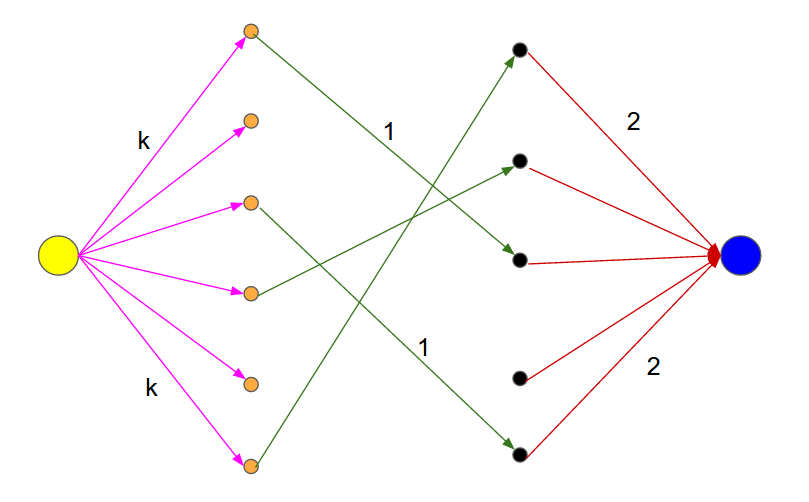
\includegraphics[width=0.5\columnwidth]{fig_one.png}
\caption{ Edge Capacities-- Pink Edges: k, Green Edges: 1, Red Edges: 2;\newline Orange Vertices: Conditions; Black Vertices: Balloons}
\label{sim}
\end{figure}
\subsubsection{Time Complexity}
Since Max-Flow takes polynomial time, and since the number of nodes($2 + n + m$) and edges($n + m + \sum_{i \in \text{Balloons}}S_i$) in this network are polynomial in input size (n,m), this algorithm is also a polynomial time algorithm.
\subsubsection{Proof of Correctness}
\textbf{Theorem: } The maximum-flow of this network (Figure \ref{sim}) is $k \times n$ \emph{iff} there exists a way in which each condition can be measured by k balloons, while each balloon measures at most two conditions.\\ \\
\textbf{Lemma 1:} Maximum Flow is $k \times n$ $ \rightarrow $ There exists a way in which each condition can be measured by k balloons, while each balloon measures at most two conditions.\\ \\
Consider the s-t cut with only s being in the left subset, then since the flow is $k \times n$ and there are n edges, each with capacity k, thus each edge has flow k. 
$$ f_e = k \hspace{5pt}\forall e=(s,i), i \in \text{Conditions}$$
Using \emph{Law of Conservation} and \emph{Principle of Integrality}, since each condition node has incoming flow k, and it has only edges of capacity 1 leaving it, therer are k edges leaving a condition node each with flow 1. This thus represents thar each measurement is taken by exactly k balloons.\\ \\
Again by \emph{Law of Conservation} and \emph{Principle of Integrality}, since each balloon node has only one outgoing edge of capacity 2, there can not be more than two edges with positive flow entering it. This , thus shows that each balloon takes atmost 2 measurements. \\ \\
\textbf{Lemma 2:} There exists a way in which each condition can be measured by k balloons $ \rightarrow $  Flow is $k \times n$ \\ \\
Since each condition node is measured by k balloons, then by \emph{Principle of Integrality}, there are k edges(each with capacity 1) leaving each condition node with flow 1 for each edge. By \emph{Law of Conservation}, since flow $1 \times k $, leaves a condition node, thus the only incoming edge must have flow k. Since all outgoing edges from source have flow k, the total flow is $k \times n$.
\subsection{Part 2}
\subsubsection{Algorithm Description}
We introduce three nodes for each condition node representing contractors (Figure \ref{dif}). Each contractor has an edge from it's corresponding condition node with capacity k-1. Let $M_{l,j}$ be the contractor node representing Contractor j ($j \in {1,2,3}$) for condition $l$($ l \in {1,2...n}$) . A balloon i produced by Contractor j has an edge from $M_{l,j}$ for all $l$ in $S_i$ with capacity 1. The rest of the network remains the same.
\begin{figure}[h!]
\centering
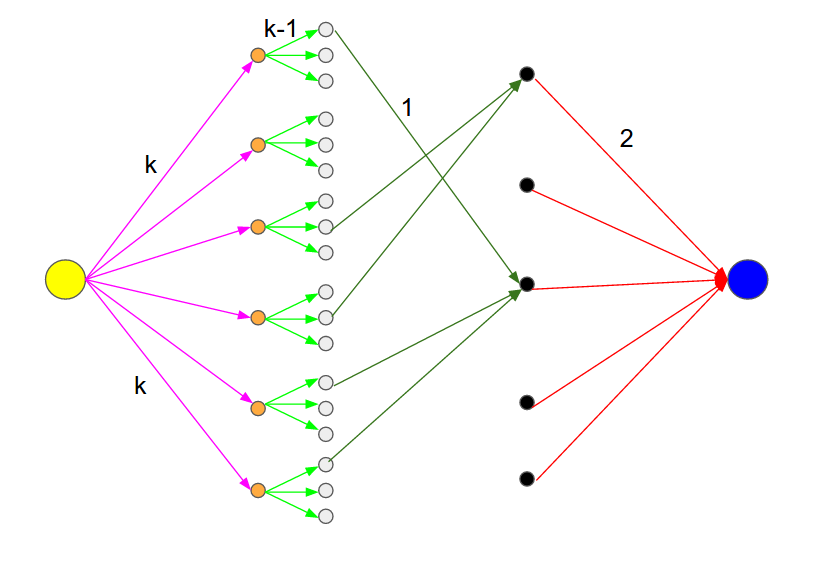
\includegraphics[width=0.5\columnwidth]{fig_dif.png}
\caption{ Edge Capacities-- Pink Edges: k, Light Green Edges: k-1, Dark Green Edges: 1, Red Edges: 2;\newline Orange Vertices: Conditions, Black Vertices: Balloons, Grey Vertices: Contractors}
\label{dif}
\end{figure}
\subsubsection{Time Complexity}
Again since Max-Flow takes polynomial time, and since the number of nodes($2 + n + m + 3 \times n$) and edges($n + m + \sum_{i \in \text{Balloons}}S_i + 3 \times n$) in this network are polynomial in input size (n,m), this algorithm is also a polynomial time algorithm.
\subsubsection{Proof of Correctness}
\textbf{Theorem: } The maximum-flow of this network (Figure \ref{sim}) is $k \times n$ \emph{iff} there exists a way in which each condition can be measured by k balloons without all the measurements being from balloons manufactured by a single contractor and each balloon measures at most two conditions.\\ \\
\textbf{Lemma 1:} Maximum Flow is $k \times n$ $ \rightarrow $ There exists a way in which each condition can be measured by k balloons without all the measurements being from balloons manufactured by a single contractor and each balloon measures at most two conditions.\\ \\
At each condition node, since incoming flow is k, by \emph{Law of Conservation} :
$$\sum_{j \in {1,2,3}}f_{e_j} = k \hspace{5pt} \forall e_j=(l,j); \forall l(\text{Condition Node})$$
Maximum capacity of each such edge is k-1. Thus, at each contractor node maximum incoming flow is k-1. Therefore, it has atmost k-1 outgoing edges with flow 1. Thus, for all conditions, there is no condition for which all k measurements come from balloons produced by single contractor. The rest of Proof follows from proof of Lemma 1 in Part 1. \\ \\
\textbf{Lemma 2:} Same as Lemma 2 in Part 2.

\section{A Social Networking Problem}
\subsection{Maximisation Problem}
Let $F_i$ to be the number of friends of Person i and $F_{i,j}$ is one if i is friend of j, otherwise 0. Now, Since we want a subset X such that number of edges in X is atleast 10 times $|X|$. This translates into:
$$ \frac{\text{Number of edges in X}}{|X|} \geq 10$$
$$ \frac{ \sum_{i \in X}F_i - \sum_{i \in X, j \in \bar{X}}F_{i,j}}{2 \times|X|} \geq 10$$
%$$ \frac{\sum_{i \in X}F_i - \sum_{i \in X, j \in \bar{X}}F_{i,j}}{2 \times|X|} \geq 20$$
Since, we have counted each internal edge $\in X$ twice in $\sum_{i \in X}F_i$ while edges from X to $\bar{X}$ have been counted once in$\sum_{i \in X}F_i$, the right hand side becomes 20 instead of 10. This now becomes the following maximisation problem:
$$ q(F) = \sum_{i \in X}F_i -  \sum_{i \in X, j \in \bar{X}}F_{i,j} - 20|X| $$

\subsection{Minimisation Problem}
Using the above equation, we can transform this into a minimisation problem, so that we can solve it using min-cut theorem :
$$ q(F) =  \textbf{F} - \sum_{i \in \bar{X}}F_i -  \sum_{i \in X, j \in \bar{X}}F_{i,j} - 20|X| $$
where $\textbf{F} = \sum_{i \in V}F_i$. Thus the minimisation problem becomes:
$$ q'(F) =  \sum_{i \in \bar{X}}F_i +  \sum_{i \in X, j \in \bar{X}}F_{i,j} + 20|X| $$
\subsection{Flow Network Construction}
Consider Figure \ref{min}, which shows the flow network(directed graph) for this problem.
\begin{figure}[h!]
\centering
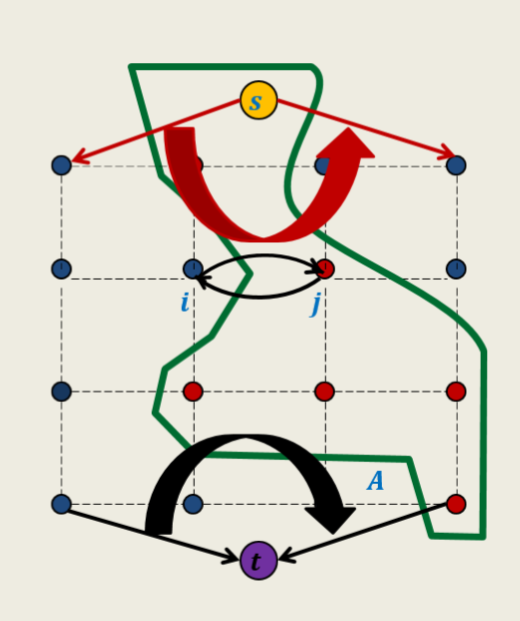
\includegraphics[width=0.5\columnwidth]{fig_minCut.png}
\caption{ Red Vertices : X , Blue Vertices : $\bar{X}$ \newline Edge Capacities: Red Edges: $F_i$ Black Edges(to sink): 20, Black Edge(between Person): 1 \newline Image Source: Lecture Slides(CS345) by Dr. Surender Baswana}
\label{min}
\end{figure}
\newline
We add a source(s) and a sink vertex (t) and assign edges and edge capacities as shown in figure. The green boundary in this graph encloses X. \\ \\
Consider the min-cut formulation of this graph:
$$ \text{Cut} = \sum_{i \in \bar{X}}c_{s,i} + \sum_{j \in X}c_{j,t} + \sum_{i \in X , j \in \bar{X}}c_{i,j}$$
$$ \text{Cut} = \sum_{i \in \bar{X}}F_i + \sum_{j \in X}20 + \sum_{i \in X , j \in \bar{X}}1$$
$$ \text{Cut} = \sum_{i \in \bar{X}}F_i +20|X| + \sum_{(i,j) E , i \in X, j \in \bar{X}}F_{i,j}$$
Now, FF algorithm will give a cut which minimises the above function which is precisely the minimisation function, we defined earlier.\\ \\
\textbf{Finding a Friend Group:} After finding min-cut, we will calculate (\textbf{F} - Min-Cut). If this is greater than 0, then we have the friend group and that group will be X, otherwise no such group exists.
\end{document}


